
\section{Physical properties}

\begin{figure}
	\centering
	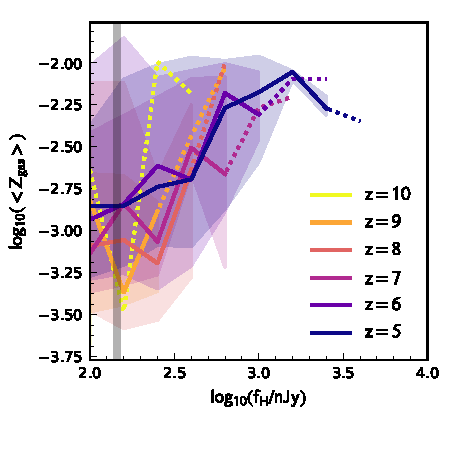
\includegraphics[width=0.45\textwidth]{figures/physical/zevo_G_Z.pdf}
	\caption{Evolution of mean gas metallicity for galaxies accessible to \euclid \: in \textsc{Flares}. The shaded region marks the centre 68\% range.}
	\label{fig:physical:gz_zevo}
\end{figure}

\begin{figure}
	\centering
	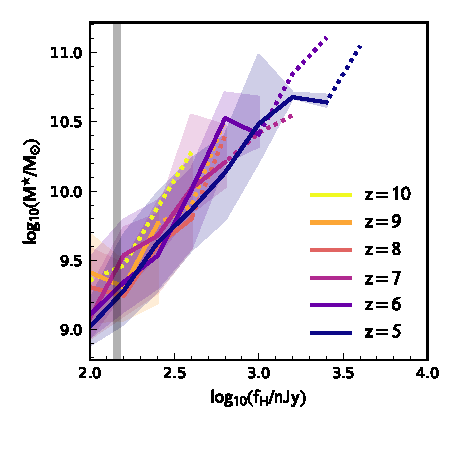
\includegraphics[width=0.45\textwidth]{figures/physical/zevo_Mstar_30.pdf}
	\caption{Evolution of stellar mass inside a 30 pkpc aperture for galaxies accessible to \euclid \: in \textsc{Flares}. The shaded region marks the centre 68\% range.}
	\label{fig:physical:mstar_zevo}
\end{figure}

\begin{figure}
	\centering
	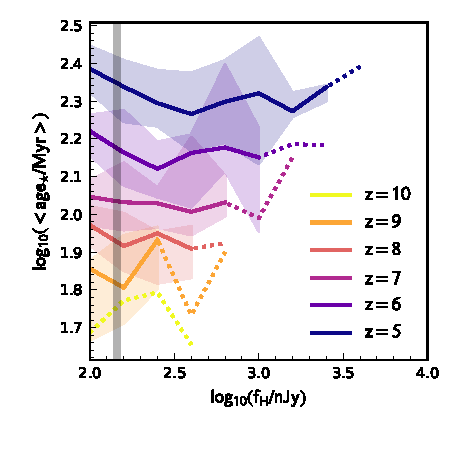
\includegraphics[width=0.45\textwidth]{figures/physical/zevo_S_Age.pdf}
	\caption{Evolution of median stellar age for galaxies accessible to \euclid \: in \textsc{Flares}. The shaded region marks the centre 68\% range.}
	\label{fig:physical:age_zevo}
\end{figure}

\begin{figure}
	\centering
	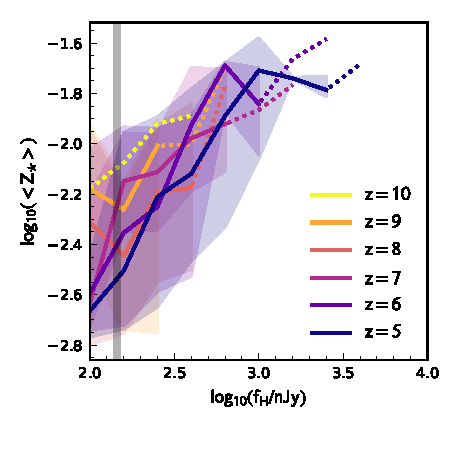
\includegraphics[width=0.45\textwidth]{figures/physical/zevo_S_Z.pdf}
	\caption{Evolution of mean stellar metallicity for galaxies accessible to \euclid \: in \textsc{Flares}. The shaded region marks the centre 68\% range.}
	\label{fig:physical:sz_zevo}
\end{figure}

\begin{figure}
	\centering
	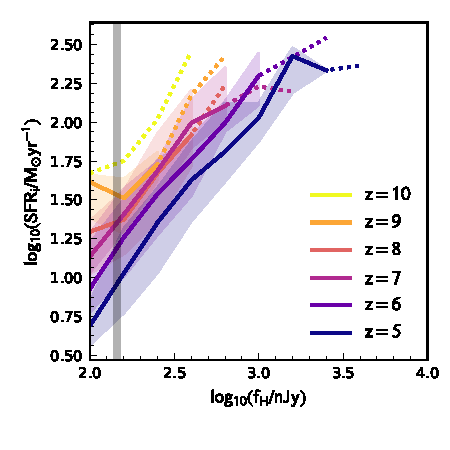
\includegraphics[width=0.45\textwidth]{figures/physical/zevo_SFR_inst_30.pdf}
	\caption{Evolution of the instantaneous star formation rate for galaxies accessible to \euclid \: in \textsc{Flares} measured within a 30 pkpc aperture. The shaded region marks the centre 68\% range.}
	\label{fig:physical:sfr_zevo_inst}
\end{figure}

\begin{figure}
	\centering
	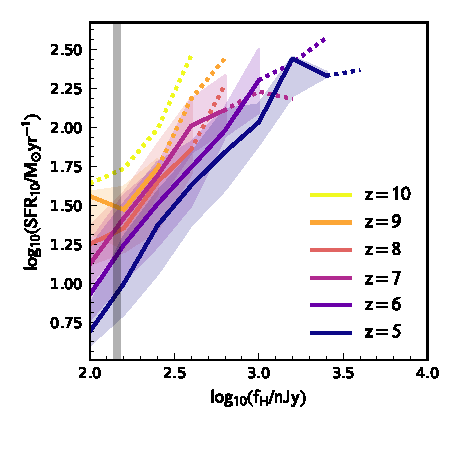
\includegraphics[width=0.45\textwidth]{figures/physical/zevo_SFR_SFR_10.pdf}
	\caption{Evolution of the star formation rate for galaxies accessible to \euclid \: in \textsc{Flares} averaged over the last 10 Myr. The shaded region marks the centre 68\% range.}
	\label{fig:physical:sfr_zevo_10}
\end{figure}

\begin{figure}
	\centering
	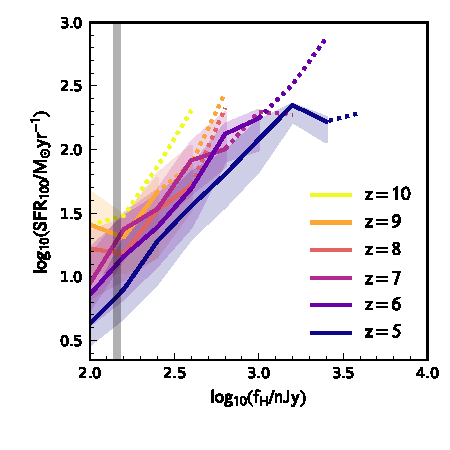
\includegraphics[width=0.45\textwidth]{figures/physical/zevo_SFR_SFR_100.pdf}
	\caption{Evolution of the star formation rate for galaxies accessible to \euclid \: in \textsc{Flares} averaged over the last 100 Myr. The shaded region marks the centre 68\% range.}
	\label{fig:physical:sfr_zevo_100}
\end{figure}
